\documentclass[aps,prl,twocolumn,10pt,superscriptaddress]{revtex4-1}
% \documentclass[aps,twocolumn,secnumarabic,balancelastpage,amsmath,amssymb,nofootinbib]{revtex4-1}
\usepackage{amsmath}
\usepackage{amssymb}
\usepackage{amsfonts}
\usepackage{color}
\usepackage{graphics}
\usepackage[pdftex]{graphicx}
\usepackage[utf8x]{inputenc}
\usepackage[colorlinks=true]{hyperref}
\usepackage{footmisc}
\usepackage{braket}

\newcommand{\ud}{\mathrm{d}}
\newcommand{\ue}{\mathrm{e}}
\newcommand{\ui}{\mathrm{i}}
\newcommand{\res}{\mathrm{Res}}
\newcommand{\Tr}{\mathrm{Tr}}
\newcommand{\dsum}{\displaystyle\sum}
\newcommand{\dprod}{\displaystyle\prod}
\newcommand{\dlim}{\displaystyle\lim}
\newcommand{\dint}{\displaystyle\int}
\newcommand{\fsno}[1]{{\!\not\!{#1}}}
\newcommand{\texp}[2]{\ensuremath{{#1}\times10^{#2}}}
\newcommand{\dexp}[2]{\ensuremath{{#1}\cdot10^{#2}}}
\newcommand{\eval}[2]{{\left.{#1}\right|_{#2}}}
\newcommand{\paren}[1]{{\left({#1}\right)}}
\newcommand{\lparen}[1]{{\left({#1}\right.}}
\newcommand{\rparen}[1]{{\left.{#1}\right)}}
\newcommand{\abs}[1]{{\left|{#1}\right|}}
\newcommand{\sqr}[1]{{\left[{#1}\right]}}
\newcommand{\crly}[1]{{\left\{{#1}\right\}}}
\newcommand{\angl}[1]{{\left\langle{#1}\right\rangle}}
\newcommand{\tpdiff}[4][{}]{{\paren{\frac{\partial^{#1} {#2}}{\partial {#3}{}^{#1}}}_{#4}}}
\newcommand{\tpsdiff}[4][{}]{{\paren{\frac{\partial^{#1}}{\partial {#3}{}^{#1}}{#2}}_{#4}}}
\newcommand{\pdiff}[3][{}]{{\frac{\partial^{#1} {#2}}{\partial {#3}{}^{#1}}}}
\newcommand{\diff}[3][{}]{{\frac{\ud^{#1} {#2}}{\ud {#3}{}^{#1}}}}
\newcommand{\psdiff}[3][{}]{{\frac{\partial^{#1}}{\partial {#3}{}^{#1}} {#2}}}
\newcommand{\sdiff}[3][{}]{{\frac{\ud^{#1}}{\ud {#3}{}^{#1}} {#2}}}
\newcommand{\tpddiff}[4][{}]{{\left(\dfrac{\partial^{#1} {#2}}{\partial {#3}{}^{#1}}\right)_{#4}}}
\newcommand{\tpsddiff}[4][{}]{{\paren{\dfrac{\partial^{#1}}{\partial {#3}{}^{#1}}{#2}}_{#4}}}
\newcommand{\pddiff}[3][{}]{{\dfrac{\partial^{#1} {#2}}{\partial {#3}{}^{#1}}}}
\newcommand{\ddiff}[3][{}]{{\dfrac{\ud^{#1} {#2}}{\ud {#3}{}^{#1}}}}
\newcommand{\psddiff}[3][{}]{{\frac{\partial^{#1}}{\partial{}^{#1} {#3}} {#2}}}
\newcommand{\sddiff}[3][{}]{{\frac{\ud^{#1}}{\ud {#3}{}^{#1}} {#2}}}
\newcommand{\eff}{ef\! f}
\newcommand{\Na}{\mathrm{Na}}
\newcommand{\Cs}{\mathrm{Cs}}
\newcommand{\fxnote}[1]{{\textbf{[#1]}}}

\newcommand{\todo}[1]{}

\ifpdf
% Ensure reproducible output
\pdfinfoomitdate=1
\pdfsuppressptexinfo=-1
\pdftrailerid{}
\hypersetup{
  pdfcreator={},
  pdfproducer={}
}
\fi

\newcommand{\harvardphysics}{\affiliation{Department of Physics, Harvard University, Cambridge, Massachusetts 02138, USA}}
\newcommand{\harvardccb}{\affiliation{Department of Chemistry and Chemical Biology, Harvard University, Cambridge, Massachusetts 02138, USA}}
\newcommand{\cua}{\affiliation{Harvard-MIT Center for Ultracold Atoms, Cambridge, Massachusetts 02138, USA}}
\newcommand{\gradstudent}{
  \harvardphysics
  \harvardccb
  \cua
}

\usepackage{xcolor}
\newcounter{TRC}
\newcommand{\TR}[1]{\textcolor{violet}{[[\stepcounter{TRC} TR\arabic{TRC}: #1]]}}

\begin{document}
% \title{Coherent optical association of atoms into a single molecule}
\title{Coherent optical creation of a single molecule}
\author{Yichao~Yu}
\email{yichaoyu@g.harvard.edu}
\gradstudent
\author{Kenneth~Wang}
\gradstudent
\author{Jonathan~D.~Hood}
\affiliation{Department of Chemistry, Purdue University, West Lafayette, Indianna, 47906, USA}
\author{Lewis~R.~B.~Picard}
\gradstudent
\author{Jessie~T.~Zhang}
\gradstudent
\author{William~B.~Cairncross}
\harvardccb
\harvardphysics
\cua
\author{Jeremy~M.~Hutson}
\affiliation{Joint Quantum Centre Durham-Newcastle, Department of Chemistry, Durham University, Durham, DH1 3LE, United Kingdom}
\author{Till Rosenband}
\harvardphysics
\author{Kang-Kuen~Ni}
\email{ni@chemistry.harvard.edu}
\harvardccb
\harvardphysics
\cua

\date{\today}

\begin{abstract}
  We report on coherent association
  of atoms into a single weakly bound NaCs molecule in an optical tweezer
  through an optical Raman transition.
  The Raman scheme uses a deeply bound electronic excited intermediate state
  to achieve a large transition dipole moment while reducing photon scattering.
  Starting from two atoms in their relative motional ground state,
  we achieve an optical transfer efficiency of $69\mathrm{\%}$.
  The molecules have a binding energy of $770.2~\mathrm{MHz}$ at $8.83(2)~\mathrm{G}$.
  This technique does not rely on Feshbach resonances or narrow excited-state lines
  and may allow a wide range of molecular species to be assembled atom-by-atom.
\end{abstract}

\maketitle

% Introduction


% 1. we want to have a diverse species to tailor to different applications including precision measurements and quantum engineering. 2. for the technique of associating atoms to form molecules, but so far all has been done with Feshbach association (before STIRAP), or in the case of Sr2, a narrow excited state. Previous work on near-threshold Raman transfer has been incoherent.
% (suggested referees: Florian Shreck and Immanual Bloch, Tanya, Deep Gupta, DeMille)

% Trapped neutral molecules, assembled in an array of optical tweezers, are a promising platform to study quantum information and quantum simulation. (more detail to add here about applications?).

Diverse species of fully quantum controlled  ultracold molecules are desired
for a variety of applications including precision measurements~\cite{
  Kondov2019,Nick_and_Ivan2017, PhysRevA.101.042504, Andreev2018,
  PhysRevLett.119.153001, hudson2011},
quantum simulations~\cite{Micheli2006, Yao2018, Wall2015, wall2015realizing},
quantum information processing~\cite{DeMille2002, Ni2018, Hudson2018, Lin2019},
and studies of ultracold chemistry~\cite{Bala2016,Hu1111,Segev2019,deJongh626}.
While many innovative approaches in the last few years
have directly cooled different species of diatomic or polyatomic molecules
below 1~mK~\cite{Norrgard2016,Anderegg2018, Mitra1366, PhysRevX.10.021049,
  PhysRevLett.121.013202, Truppe2017},
the highest phase-space-density gas~\cite{Demarco2018} and
% the coldest
trapped individual molecules~\cite{Zhang2020,He331}
have been achieved through the association of ultracold atoms.
% (any place to cite molecular ion work?)
% Citations are not complete. Add them as you see fit.

Molecular association of ultracold atoms takes advantage of the cooling and trapping techniques
that have been developed for atoms.
Associating atoms into deeply bound molecules is challenging
because of the small wavefunction overlap between the free-atom and molecular states
and the release of a large amount of binding energy.
A widely used method of overcoming these challenges is to associate atom pairs
into weakly bound molecules first,
and then transfer the molecules from this single internal state
to a desired rovibrational and electronic state,
releasing the binding energy by stimulated emission~\cite{Danzl2008, Ni2008, Lang2008,
  Takekoshi2014, Molony2014, Park2015, Guo2016, Kondov2019, Voges2020}.
So far, molecular association has generally been achieved by magnetoassociation
through a magnetic Feshbach scattering resonance.
Exceptions include Sr$_2$, where narrow linewidth ($\sim 20~\mathrm{kHz}$) excited states
are available and optical association can be driven coherently~\cite{Reinaudi2012,Stellmer2012},
and $^{87}$Rb$^{85}$Rb,
where there are molecular states bound by $1-2~\mathrm{MHz}$~\cite{He331}.
With these requirements, molecules involving non-magnetic atoms
or atoms without narrow intercombination lines remain difficult to associate.
% These requirements limit the generality of previous association techniques.
% The requirement of a Feshbach resonance or a MHz-level binding energy bound state to enhance atom-to-molecule wavefunction overlap or the existence of narrow excited-state lines limits the generality of previous association techniques. % to more diverse species.



Here, we demonstrate coherent association of an atom pair to a weakly bound molecule
by two-photon optical Raman transfer via an electronic excited state,
as shown in Fig.~\ref{f-theory}a.
The scheme does not rely on a Feshbach resonance,
molecular states bound by a few~MHz, or a narrow excited state.
The resulting single molecule is in a well-defined internal quantum state
and predominantly in its motional ground state.
A vibrational state of the electronic excited state $\mathrm{c^3\Sigma^+}(\Omega = 1)$
serves as the intermediate state in the Raman scheme,
and is chosen to minimize photon scattering during Raman Rabi oscillations.
To reduce photon scattering and sensitivity to laser intensity noise further,
we choose the initial and final states to balance the two Rabi frequencies as much as possible.
This system-independent approach creates molecules atom-by-atom with full quantum state control.


\begin{figure*}
  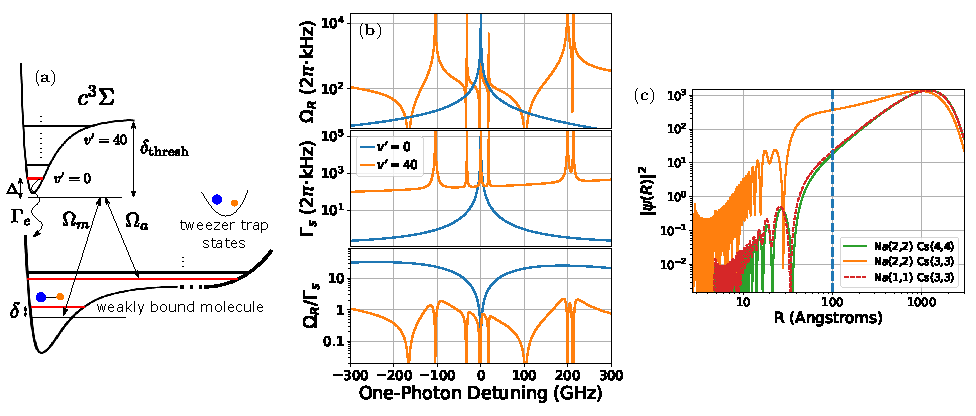
\includegraphics[width=\textwidth]{imgs/fig-theory.pdf}
  \caption{Optical creation of single molecule from single atoms in tweezer.
    (a) Schematic of the optical transition from an atom pair to a weakly bound molecule.
    The initial state is the relative motional ground state between the two atoms
    and the final state is the first molecular bound state.
    The transition is driven by a pair of laser frequencies whose difference matches the binding energy
    of the molecule.
    The lasers are detuned from an excited molecular state in the $\mathrm{c^3\Sigma}$ potential
    by $\Delta$ in order to suppress scattering during the transfer.
    (b) Comparison between weakly-bound and deeply-bound intermediate excited state
    for the Raman transition.
    The deeply bound excited state (blue lines $v'=0$)
    has a larger ratio of Raman Rabi frequency to scattering rate
    compared to the weakly bound excited state (orange lines $v'=40$) at a most detuning.
    (c) Enhancement of the short-range wavefunction.
    The large scattering length for the $\Na(2,2),\Cs(3,3)$ state creates an interaction shift
    comparable to the axial trapping frequency.
    This causes a significant change in the relative wavefunction, especially at short
    internuclear distance ($R$).
    Compared to other spin states with weaker interaction,
    the wavefunction at short distance ($R<100\ \text{\AA}$, left of the dashed line)
    is significantly enhanced.
    \label{f-theory}
  }
\end{figure*}

\begin{figure}
  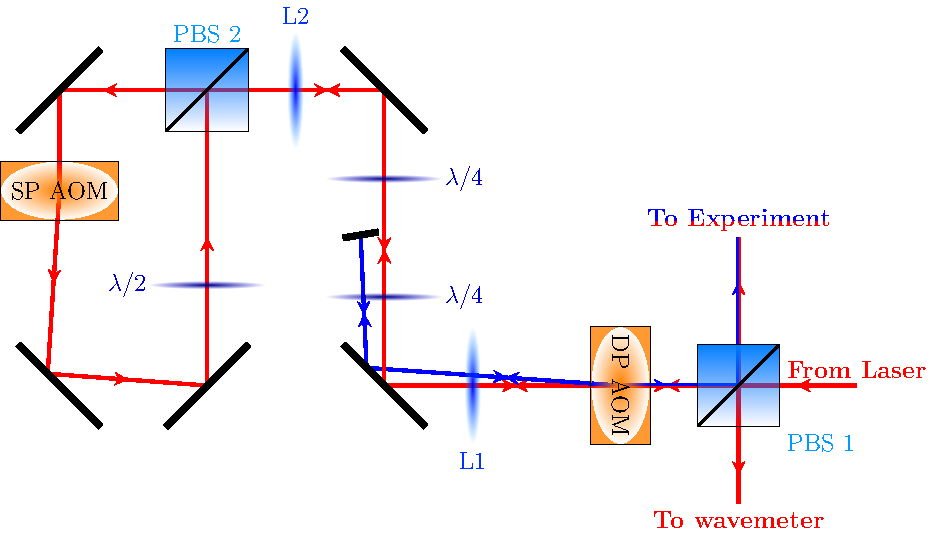
\includegraphics[width=0.5\textwidth]{imgs/raman_spectroscopy_raman_beampath.pdf}
  \caption{
    Beampath for generating the frequency for Raman transition in the tweezer.
    (Some mirrors and other optics used for alignment are not included.)
    The two ASE filters before and after the fibers are also shown. The laser source is a fiber amplifier seeded by a external cavity diode laser. 
    The red beam path is the $0$-th order of the double pass~(DP) AOM
    which is used for the tweezer.
    When the double-pass~(DP) AOM is turned on, some power is redirected to the first order
    (blue beam path) which generates the required frequency different to drive
    the Raman transition. The two frequencies are recombined on the DP AOM.
    The $0$-th order light is shifted by another single pass~(SP) AOM
    running on a different frequency before recombining.
    Without this AOM, the leak light from the DP AOM will be at the same frequency
    as the $0$-th order light which can cause a significant power fluctuation
    due to interference.
    The experiment typically start with the SP AOM on and the DP AOM off.
    When driving the Raman transition, the powers on both AOMs are ramped simultaneously
    to achieve the desired power at both frequencies.
    \label{f-beampath}
  }
\end{figure}


The optical Raman transfer is illustrated
by the idealized three-level system shown in Fig.~\ref{f-theory}a,
where the initial atomic state and the target weakly bound molecular state are coupled to an intermediate state by two lasers with Rabi frequencies $\Omega_a$ and $\Omega_m$ with one-photon detuning $ \Delta $, and all Rabi frequencies are population oscillation frequencies.  %(Ultimately, we calculate with contribution of all vibrational states of the excited electronic potential, $\mathrm{c^3\Sigma^+}$)
The transfer Raman Rabi Rate is given by $\Omega_a\Omega_m / (2\Delta)$~\cite{Wineland2003}.
% , is accompanied by a photon scattering rate $\Gamma_e (\Omega_a^2 + \Omega_m^2)/4\Delta^2$
% $\Gamma_e \Omega^2 / 4\Delta^2 $, where $ \Gamma_e $ is the excited state linewidth
Unlike Raman transitions in atoms, the two Rabi frequencies are greatly imbalanced ($\Omega_a/\Omega_m \ll 1$) %. Since $ \Omega_m $ is generally much larger than $ \Omega_a $
due to the small wavefunction overlap between the atomic state and the intermediate state, %the atomic state and the excited molecular state,
and scattering losses are dominated by the final state. Furthermore, the energy difference between the atomic state and target molecular state is small ($ < 1~\mathrm{GHz} $) compared to the single-photon detuning $ \Delta $ of $80$ to $200$~GHz, causing the target molecular state to scatter both beams nearly equally with a total rate $ \Gamma_e \Omega_m^2 / (2\Delta^2)$, where $ \Gamma_e $ is the excited-state linewidth~\footnote{The two beams have equal power to maximize the Raman Rabi rate at fixed total power, resulting in a factor of 2 for scattering two beams.}.
In this idealized treatment, the ratio between the Raman Rabi frequency and the scattering rate is $ \Omega_a/\Omega_m \times \Delta/\Gamma_e $, which limits the transfer efficiency into the molecular state. At the same time, the intensity-stability requirement is determined by the ratio of Raman Rabi frequency to Stark shift ($\Omega_a/\Omega_m$)~\footnote{There is an additional factor of 2, with both beams at equal power,
  to account for the Stark shift caused by both beams.}. Notably, both figures of merit improve with a larger ratio $\Omega_a/\Omega_m$. %, depends on the ratio of the two matrix elements and how far detuned the laser is from the transition in units of the linewidth.
To ensure a coherent process, a detuning as large as possible, while maintaining a realistic Raman Rabi frequency, is preferred \TR{Mention 2-photon here?}. %However, the detuning cannot be too large, since that will reduce the Raman Rabi frequency.

Earlier experiments used weakly bound excited states as the intermediate state
in the Raman transition to ensure a large Raman Rabi frequency~\cite{Wynar2000,Rom2004}.
However, a complete picture includes both the many vibrational levels
of the excited electronic state and the atomic continuum.
The total scattering rate and Raman Rabi rate become a sum of the scattering rates
and Raman Rabi rates over all possible intermediate states.
As there is large overlap between the target molecular state and weakly bound excited states, intermediate states that are closer to the dissociation threshold result in a large scattering rate.
% in large incoherence and loss to other molecular states.
This scattering is approximately proportional to $1/\delta_{\mathrm{thresh}}^2$,
where $\delta_{\mathrm{thresh}}$ is the detuning from the dissociation threshold,
which is smaller for intermediate states that are deeply bound \footnote{See Supplementary Material}. \TR{Cite supplement or maybe Fig. S1 can go into Fig. 1b since it shows $\Gamma_s\sim \delta_{thresh}^{-2}$ nicely.}.


We optimize over intermediate states by calculating the Raman Rabi frequency $\Omega_R$
and scattering rate $\Gamma_s$ at different detunings from the atomic threshold,
taking into account of all states of
8 excited molecular potentials~\cite{Korek2007, Grochola2011, Zaharova2009, Grochola2010, Zabawa2012}
and the continuum~\cite{Liu2017}.
This calculation shows that the figure of merit $\Omega_R/\Gamma_s$
can be larger for more deeply bound states compared to weakly bound states
at a cost of a smaller transfer rate $\Omega_R$, as shown in Fig.~\ref{f-theory}b;
see Supplementary Material for details.
As a result, we choose the $v'=0$ level of $\mathrm{c^3\Sigma^+}(\Omega = 1)$
as the intermediate state near which to drive Raman transitions.

In addition to the intermediate state,
the choice of initial and final Zeeman and hyperfine states affects the single-photon rates $\Omega_a$ and $\Omega_m$.
Due to the small extent of the intermediate-state wavefunction
compared to that of the trapped atoms,
$\Omega_a$ is approximately proportional to
the amplitude of the relative atomic wavefunction at short distance,
within the range of the molecular potential.
To increase this amplitude, one can increase the external confinement of atom pairs.
In a harmonic approximation
the short-range amplitude is proportional to $ \omega_{\text{trap}}^{3/4} $ or $P^{3/8}$,
where $ \omega_{\text{trap}} $ is the trap frequency and $P$ is the optical power in the tweezer trap \cite{Mies2000} with a fixed beam waist. However, additional power may not be available and also leads to additional undesired scattering.
Alternatively, one can choose an atomic pair state with a large scattering length
(positive or negative).
For such states, the amplitude of the relative atomic wavefunction is substantially enhanced
at short range, as shown in Fig.~\ref{f-theory}c.
% The increase in the coupling is proportional to (quote/cite Olive's equation?).
For our system of Na and Cs atoms,
we choose a spin-state combination $\ket{\uparrow_{\Na} \downarrow_{\Cs}}\equiv \ket{f=2,m_f=2}_{\Na}\ket{f=3,m_f=3}_{\Cs}$ that has a large and negative scattering length of
$a(\uparrow_{\Na} \downarrow_{\Cs}) \approx -700a_0$~\cite{Hood2019}.
All other stable spin combinations give smaller scattering lengths ($<~50~a_0$).
% We denote the possible hyperfine states of the atoms as $ \ket{\uparrow_{\Cs}} = \ket{f=4,m_f=4}_{\Cs}, \ket{\downarrow_{\Cs}} = \ket{f=3,m_f=3}_{\Cs}, \ket{\uparrow_{\Na}} = \ket{f=2,m_f=2}_{\Na}, $ and $ \ket{\downarrow_{\Na}} = \ket{f=1,m_f=1}_{\Na}$. Among the stable spin combinations, $\ket{\uparrow_{\Na}\uparrow_{\Cs}}$ and $\ket{\downarrow_{\Na}\downarrow_{\Cs}} $ both have small scattering lengths of $ 30.4a_0 $, and $ 13.7a_0 $ respectively, but the $\ket{\uparrow_{\Na} \downarrow_{\Cs}} $ combination has a large and negative scattering length of $ a(\uparrow_{\Na} \downarrow_{\Cs}) = -693.8a_0 $ (interaction shift $\approx$ binding?)~\cite{Hood2019}.

To identify a suitable target molecular state, we carry out coupled-channel calculations of the near-threshold bound states, as described in the Supplemental Material.
Choosing a bound state with similar spin character to the atomic state  minimizes the sensitivity of the transition frequency to magnetic field.
A suitable state with this character is predicted about 763 MHz below the $\ket{\uparrow_{\Na} \downarrow_{\Cs}}$ threshold and the ratio $\Omega_a/\Omega_m$ increases to about 0.013.
% The coupled-channel calculations show that this target molecular state has lower overlap with the intermediate state, compared to bound states from other hyperfine combinations.
% For the target molecular state, the spin state is ideally similar to the initial spin state in order to minimize sensitivity to the magnetic field.
% We find a target spin state predominantly in the initial spin state
% that also has the advantage of having a reduced sensitivity
% to laser intensity noise because of a larger %$\Omega_a/\Omega_b$ as compared to other states.
% This reduces the intensity stability requirement to $5~\mathrm{\%}$
% instead of $0.3~\mathrm{\%}$ which is typical for other states.
% In addition to the increased atomic coupling, $ \Omega_a $,
% Coupled-channel calculations show that this target molecular state with similar spin composition also has reduced Rabi frequency, $ \Omega_m $, with the intermediate state when compared to bound states of the other spin compositions.
% $\ket{\uparrow_{\Na}\uparrow_{\Cs}}$ and $\ket{\downarrow_{\Na}\downarrow_{\Cs}} $ bound states.
Compared to $\Omega_a/\Omega_m \approx 0.003$
for other combinations, this relaxes the intensity stability requirement to the percent level and enhances the Raman Rabi frequency. % Thus, instead of a required intensity stability of $0.3 ~\mathrm{\%} $ for the 4422 or 3311 combination, the 3322 combination only requires the intensity to be stabilized to $ 5~\mathrm{\%} $.
% Thus, we choose the $\ket{\uparrow_{\Na} \downarrow_{\Cs}}$ spin combination as our initial state and drive to the first bound state for the $\ket{\uparrow_{\Na} \downarrow_{\Cs}}$ spin combination.
% \textcolor{blue}{(clean up the paragraph some more).} %(We might want to mention that those ratios are for 80 kHz spherical trap if we want to give more details about the coupled-channel calculation anywhere...)

% In additional to the final and the excited state, it is also important to select the an initial atomic state in order to improve the coupling.
\begin{figure}[ht!]
  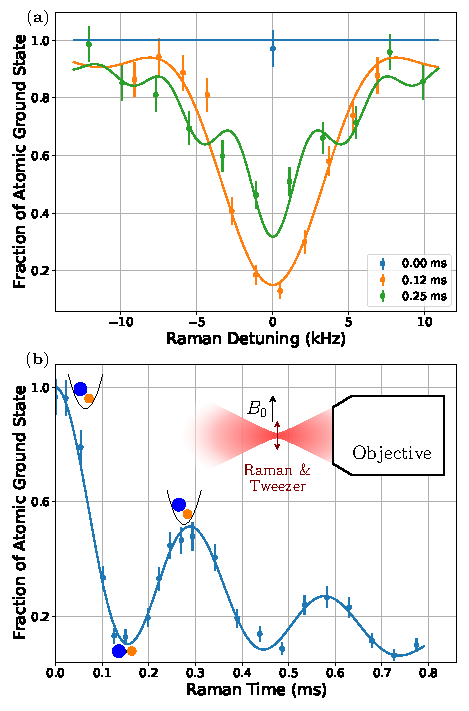
\includegraphics[width=0.48\textwidth]{imgs/fig-raman.pdf}
  \caption{Coherent transfer of atoms to molecules.  The molecular state is dark to the imaging step and corresponds to zero signal.
    (a) Raman difference frequency scans for various durations showing the resonance as a frequency offset from $770.2$~MHz, near the calculated value of $763$~MHz.
    (b) Raman pulse-length scan on resonance.
    A decaying Rabi oscillation shows the coherence of
    the Raman transfer process.
    A model is fitted to (a) and (b) to determine
    the Raman Rabi frequency and loss rates.
    \emph{Inset:} Geometry and polarization of trap and Raman beam relative to the magnetic field.
    The X.yy~mW beam is focused to a waist of $0.9~\mathrm{\mu m}$
    that confines the atoms and molecule.
    A perpendicular $B_0=8.83(2)~\mathrm{G}$ magnetic field 
    defines the quantization axis and the atoms experience predominantly $\pi$-polarized light.
    \label{f-raman}}
\end{figure}

%% Preparation
Experimentally, we first prepare two atoms in a well-defined external and internal quantum state
by using techniques developed previously~\cite{Liu2018, Liu2019, Wang2019}.
In brief, the experimental cycle begins by stochastically loading a single ${}^{23}\Na$ atom
and a single ${}^{133}\Cs$ atom into separate optical tweezers.
The atoms are initially imaged to distinguish between loading of two atoms,
one atom (Na or Cs), or no atom to be able to post-select from the experimental results
based on the initial loading condition.
After imaging, we turn on a $8.83(2)~\mathrm{G}$ magnetic field to define the quantization axis
for the state preparation and molecule formation steps.
Raman sideband cooling is then applied to prepare both atoms simultaneously
in the 3-dimensional motional ground state of their optical tweezers, leaving the atoms in the spin state~$\ket{\uparrow_{\Na}\uparrow_{\Cs}}\equiv \ket{f=2,m_f=2}_{\Na}\ket{f=4,m_f=4}_{\Cs}$,
which has a small scattering length.
The weak two-atom interaction allows merging of the two tweezers with minimum pertubation so that they remain in the motional ground state.

% After preparing the Na and Cs atoms in the same tweezer in a single quantum state,
Next, we drive the atoms into spin combination $\ket{\uparrow_{\Na} \downarrow_{\Cs}}$ with a large scattering length
by performing a Cs spin flip while taking into account
the $-30.7~\mathrm{kHz}$ interaction shift~\cite{Hood2019}.
This is the initial atomic state for Raman transfer.
The spin flip selectively transfers atoms in the relative motional ground state,
removing any background from atoms in excited motional states
\footnote{This interaction shift is larger than the differential axial trapping frequency
  between Na and Cs atoms, which decouples the relative and center of mass motional state
  and improves the robustness of our preparation of the relative motional ground state.}.
For the experiment reported here,
$31\mathrm{\%}$ of initial two-atom population is transferred.
% of two atoms loaded in separate optical tweezers.\textcolor{red}{I also find this part of the sentence confusing.  can you say this more concisely?}\todo{}
% The stronger interaction in this spin state also enhances the atomic wavefunction at short range and increases its overlap with the intermediate molecular state used for our Raman transfer..

%% Transfer scheme
% After the atoms are prepared in the $\ket{\uparrow_{\Na}\uparrow_{\Cs}} $ hyperfine combination, we then perform the Raman transfer.
To transfer the atom pair into the target weakly bound molecular state,
we modulate the tweezer beam with a second frequency near $770$~MHz, as shown in Fig.~\ref{f-beampath}.
The dual use of the tweezer beam for confinement and Raman transfer not only minimizes photon scattering,
but also allows a tight focus to minimize the transfer duration. A tweezer frequency far detuned (by $-151~\mathrm{GHz}$) from the 3 observed rotational~\TR{spectral?} lines at $v' = 0 $ reduces resonant scattering~\cite{Liu2019}.
%Furthermore, two filters, each with a linewidth (FWHM) of $50~\mathrm{GHz}$,
%clean the laser spectrum and prevent broadband noise from causing unwanted excitation.
%As shown in Fig.~\ref{f-beampath}, one filter immediately follows the laser, while the second filter precedes the microscope objective for final cleanup of the laser spectrum.
%The filters reduce photon scattering rate by a factor of $2$ (\textcolor{red}{KW: Since we mention this again later when we explore the causes of our lower than expected transfer efficiency, do we need to mention this reduction here? or the possible causes?}). While we have not fully characterized the sources
%of broadband noise, possibilities include amplified spontaneous emission (ASE) from the laser and fiber nonlinearities.
% After the total tweezer power is set to the desired value,
% we smoothly ramp down the power of one frequency in the tweezer
% while simultaneously ramping up the power of the other frequency
% so that the total tweezer power remains unchanged.
% Both frequencies are kept on for a specified duration before the process is reversed
% and the tweezer returns to a single frequency.~\TR{???}

% found the spectral purity of the laser for Raman beams to be critical for achieving a higher transfer efficiency.
% The tweezer/Raman beams are generated by a fiber amplifier seeded with a $1037~\mathrm{nm}$ external cavity diode laser.
% by amplifying a $1037~\mathrm{nm}$ external cavity diode laser (ECDL) with a fiber amplifier,
% The diode laser produces the desired frequency on top of a broad band amplified spontaneous emission (ASE).  We use a Bragg grating with a line width (FWHM) of $50~\mathrm{GHz}$ to clean up the laser spectrum and found it reduces the scattering rate by at least a factor of $2$
% for a particular single-photon detuning.

% in addition to the desired frequency. This increases the scattering rate due to coupling to other excited states.



%% Experiment condition/resonance

\begin{figure}[t!]
  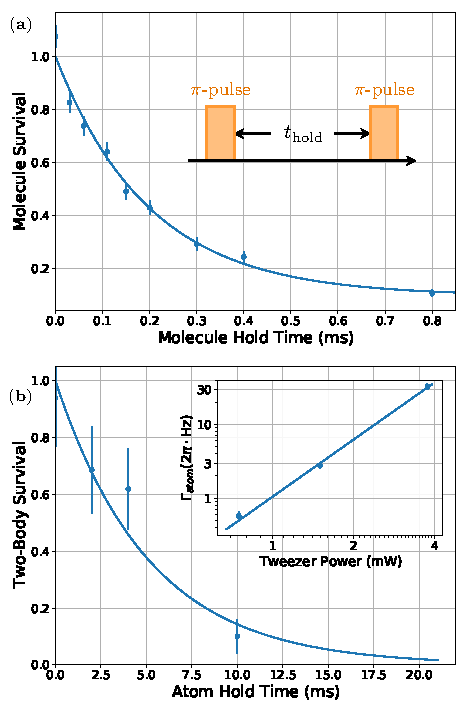
\includegraphics[width=0.48\textwidth]{imgs/fig-lifetime.pdf}
  \caption{
    (a) Direct measurement of molecule lifetime with about $3.75~\mathrm{mW}$ optical power.
    Molecule survival is detected by dissociating back to atoms via a second Raman transition.
    The lifetime is consistent with the $0.199(9)~\mathrm{ms}$
    measured from the Raman transition data.
    Inset: pulse sequence for the lifetime measurement.
    (b) Two-body atom lifetime of $5(1)~\mathrm{ms}$
    in a trap of depth $3.75~\mathrm{mW}$ caused by off-resonance photoassociation.
    This is used to improve the fitting of the Raman transfer data.
    Inset: Atomic scattering rate scales as
    $P_\textrm{tweezer}^{2.58}\times\!2\pi\!\times29.3(17)~\mathrm{mHz/mW^{2.58}}$ on a log-log scale;
    this is consistent with a two-photon scattering process.
    We have not measured a clear dependency of the loss rate on the tweezer detuning.
    \label{f-lifetime}}
\end{figure}

Figure~\ref{f-raman} shows a Fourier-limited resonance together with Rabi oscillations between the atomic and molecular states.
% (We can maybe add information about the prediction here?)
%% Prediction
% This excited state used in the Raman transition was measured in our previous experiment using photoassociation to be at $288560 GHz$ from our atomic state. The ground molecular state has not been observed previously in experimentally. Based on our measurement of FB resonance, interaction shift and the binding energy of the 4422 bound state. Theory prediction was at $770.1 MHz$.
% The background level of $31~\mathrm{\%}$ corresponds to the probability of preparing the two atoms in the relative motional ground state.
% When the atoms are transferred into the molecule state by the Raman transition, there is a decrease in the two body survival since the resulting molecule is dark to our imaging sequence. % directly detected by our imaging step.
A decaying Rabi oscillation with frequency $2\pi\times3.28(4)~\mathrm{kHz}$ fitted to the data suggests that
$69~\mathrm{\%}$ of atoms initially in the relative motional ground state are transferred into the molecular state after a $\pi$-pulse. Over $60\%$ of the molecules are in the motional ground state (both relative and center of mass), inferred from independent Raman sideband thermometry measurements of the atoms.

\begin{figure*}
  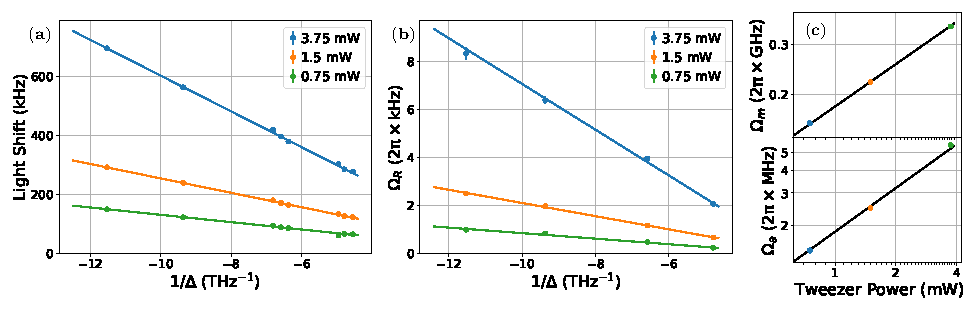
\includegraphics[width=\textwidth]{imgs/fig-det.pdf}
  \caption{Raman transition parameters as a function of tweezer power and detuning.
    (a) The Raman resonance fitted by $a_P+b_P/\Delta$, where
    $a_P$ and $b_P=(\Omega_a^2-\Omega_m^2)/2$
    are the power ($P$) dependent background and $v'=0$ contributions
    to the light shift and
    $\Delta\equiv2\pi\times\paren{f_0 - f_{\mathrm{tweezer}}}$ is the detuning from
    the $v'=0$ resonance frequency $f_0$.
    $a_P$ is fitted to a model including linear and small quadratic light shift
    \todo{which assumes $\Omega_m\gg\Omega_a$} to obtain the Raman resonance frequency
    at zero tweezer power $\omega_{R0}=2\pi\times770.1969(2)~\mathrm{MHz}$ where the statistical uncertainty is shown.
    (b) Raman Rabi frequency ($\Omega_R$) fitted to $c_P+d_P/\Delta$, where
    $c_P$ and $d_P=\Omega_a\Omega_m/2$
    are the background and $v'=0$ contributions that scale as $P^{1.29}$ with optical power.
    The detuning is calculated from the PA frequency fitted in (a). Fit parameters are listed in Table~\ref{tab:f-det:fit}.
    (c) Tweezer power dependency of $\Omega_m$ (top) and $\Omega_a$ (bottom) calculated from
    $b_P$ and $d_P$ on a log-log scale showing approximate $P^{0.5}$ scaling of $\Omega_m$ and
    $P^{0.79}$ scaling of $\Omega_a$. [[TR: There should be a gap between (c) top and bottom.]
    \label{f-det}}
\end{figure*}

To better understand the details and limitations of the Raman transfer process, we measured the properties of the two-photon resonance as a function of tweezer power and single-photon detuning.
Known dependencies of the light shift and Raman Rabi frequency on detuning $\Delta$ allow experimental determination of the Rabi frequencies
$ \Omega_a $ and $\Omega_m$ whose ratio critically affects the transfer efficiency.
Both the light shift and Raman Rabi frequency follow a $1/\Delta$ slope as shown in Fig.~\ref{f-det}a, b and include a constant offset that we attribute to coupling to other excited states that are further away in energy.
The $1/\Delta$ components, due to the nearby $v'=0$ intermediate state, determine $\Omega_m $ and $ \Omega_a $ in from the fit coefficients, as shown in Table~\ref{tab:f-det:fit}.

\begin{table}[ht]
  \centering
  \begin{tabular}{|c|c|c|c|}
    $P~(\mathrm{mW})$&$0.75$&$1.5$&$3.75$\\\hline
    $f_{\mathrm{PA}0}~(\mathrm{GHz})$&\multicolumn{3}{|c|}{$288711.8$}\\\hline
    $a~(\mathrm{2\pi\times MHz})$&$770.20452(6)$&$770.2081(1)$&$770.1943(3)$\\
    $b~(\mathrm{4\pi^2\times MHz\cdot GHz})$&$-12.46(2)$&$-24.44(3)$&$-60.66(8)$\\\hline
    $c~(\mathrm{2\pi\times kHz})$&$0.29(2)$&$0.63(4)$&$2.4(2)$\\
    $d~(\mathrm{4\pi^2\times MHz\cdot GHz})$&$0.115(4)$&$0.275(6)$&$0.95(3)$\\ \hline
    $\Omega_R~(\mathrm{2\pi\times kHz})$ & & & X.YY \\
    $\Omega_m~(\mathrm{2\pi\times MHz})$ & & & 348.3(3) \\
    $\Omega_a~(\mathrm{2\pi\times kHz})$ & & & 5.5(2)
  \end{tabular}
  \caption{Fitting results for Fig.~\ref{f-det}(a,b). $\Omega_R$ is reported at $-151~\mathrm{GHz}$ detuning from the $v' = 0$ state.  The coefficients $\Omega_m$ and $\Omega_a$ are in broad agreement with our calculation and their ratio $63$ is near the theory prediction of $78$.  The measured Rabi rate $\Omega_R$ is ZZ~\% of $\Omega_m \Omega_a/(2\Delta)$ due to interference from further-detuned Raman processes.
    \label{tab:f-det:fit}}
\end{table}

We perform the experiment at various tweezer powers to extract the power dependence of $ \Omega_m $ and $ \Omega_a $, as shown in Fig.~\ref{f-det}c. $ \Omega_m $ scales like $ P^{1/2} $ as expected. As discussed previously, the scaling of $ \Omega_a $ is $P^{7/8}$ for weakly interacting particles.
However, due to the strong interaction between the two atoms in the $\ket{\uparrow_{\text{Na}}\downarrow_{\text{Cs}}}$ state, this approximation breaks down.
Coupled-channel calculations show that the wavefunction scaling
is well approximated by $P^{0.29}$ within the range of confinement in our experiment and the expected scaling of $ \Omega_a \propto P^{0.79} $ agrees with the data.
% At $3.75~\mathrm{mW}$ tweezer power, we measured $ \Omega_m = 2\pi \times 348.3(3)~\mathrm{MHz}$ and $ \Omega_a = 2\pi\times 5.5(2)~\mathrm{MHz}$, resulting in a
% The measured $ \Omega_m/\Omega_a$ ratio of $ 63 $ is close to the theory prediction of $77.7$~(Table~\ref{tab:rabi_freqs}).
% Therefore, the matrix element ratio is not the cause of our lower than expected transfer efficiency.

% We observe that the resonance frequency depends linearly on the tweezer power due to the differential light shift between the atomic and molecular state.
% From these measurements, we can extract a $\Omega_m$ of


% In order to calculate the ratio $\Omega_m/\Omega_a$,
% we now need to extract $ \Omega_a $.
% We do this by measuring the dependence of the Raman Rabi frequency on power and detuning.
% which depends on both $\Omega_m$ and $\Omega_a$.
% The Raman Rabi frequency shows a non-linear dependency on the tweezer power
% due to the change in the atomic wavefunction caused by
% tighter confinement at higher power, as shown in Fig.~\ref{f-det}b.

% Combined with the standard intensity factor, the Raman Rabi frequency should scale as $P^{1.29}$,
% which fits well to our experimental result, as shown in Fig.~\ref{f-det}b.
% Similar to the light shift, the detuning dependency of the Raman Rabi frequency
% is determined by a constant background component and
% a $v'=0$ component that scales as $1/\Delta$.
% The $v'=0$ component of the Raman Rabi frequency at our detuning is
% $2\pi\times1.10(2)~\mathrm{kHz\cdot mW^{-1.29}}$,
% or $2\pi \times 6.08(9)~\mathrm{kHz}$ at $3.75~\mathrm{mW}$ %tweezer power.
% Together with the $\Omega_m$ measured above, the Rabi frequency, $\Omega_a$, is
% $2\pi\times 5.5(2)~\mathrm{MHz}$.
% This gives a matrix-element ratio $\Omega_m/\Omega_a$ of $63(3)$,
% which is close to the theory prediction of $77.7$~(Table~\ref{tab:rabi_freqs}).

% Theory numbers
% $2\pi \times 15.3~\mathrm{kHz}$
% $ 2\pi \times 533~\mathrm{Hz}$
% $2\pi \times 573 ~\mathrm{MHz}$
% $2\pi \times 7.37 ~\mathrm{MHz}$

% With the contribution of the $ v' = 0 $ state to the Raman Rabi frequency and scattering investigated,
% We now consider the background effects from other states with larger single-photon detuning.
% In the Raman Rabi frequency fit,
% the fitted background is of opposite sign from the Raman Rabi frequency
% for single-photon detunings red of the $v' = 0 $ transition.
% Thus, this background reduces the Raman Rabi frequency by about $30~\mathrm{\%}$
% at the current detuning.
% However, this difference is not enough to explain the discrapancy of more than a factor of $10$
% present in the experiment.
% Due to the change in sign of the Raman Rabi frequency as a function of detuning
% when crossing a resonance, the same background will increase the Raman Rabi frequency
% for positive detunings from the $v' = 0$ transition.
% Unfortunately, we observe additional nearby excited states
% belonging to a different electronically excited state at higher frequencies
% which prevent the blue side of the transition from being be usable for the Raman transition.

The measured single-photon Rabi frequencies of Table~I are in broad agreement with calculations (see Supplementary Materials). Known single-photon scattering rates of Na and Cs atoms together with an independent measurement (via photoassociation spectroscopy) of the $v'=0$ excited state natural linewidth of no more than $50~\mathrm{MHz}$ indicate that single-photon scattering from the molecular or atomic state do not explain the decoherence in Fig. 3b~\TR{long sentence}.  Below, we further investigate the loss of coherence.

\todo{change scattering to decoherence? since the fluctuation of light shift
  does not lead to scattering but only decherence.}
% These results suggest that the decoherence or loss we observe during the Raman transition
% comes from either a higher background scattering rate of an unknown source
% or a different intrinsic or technical source for which we have not accounted for.
Raman transfer efficiency is limited by the molecular lifetime, together with a reduction in the Raman Rabi frequency due to destructive interference with intermediate states beyond v'=0 (see Table~~\ref{tab:f-det:fit}).
The lifetime is measured directly by preparing the molecule with a $\pi$-pulse,
followed after a variable delay by a second dissociating $\pi$-pulse.
The result in Fig.~\ref{f-lifetime}a shows a molecular lifetime of $0.199(9)~\mathrm{ms}$,
consistent with the decay of the Rabi oscillation in Fig.~\ref{f-raman}b.
Preliminary experiments and theoretical considerations indicate that the molecular lifetime may be limited by two-photon coupling to the atomic continuum~\cite{YichaoYu}.  Atom loss is shown to be small in Fig.~\ref{f-lifetime} by measuring the one- and
two-body lifetimes of the atoms directly without the second Raman frequency.  In principle, destructive interference that reduces the Raman Rabi rate for negative detunings $\Delta$ changes to constructive interference for positive detunings, but additional molecular resonances made the positive region unusable.  Separately we observe a decrease in coherence by a factor of 2 without laser spectrum filters,
suggesting that spectral impurity of the laser can be a significant source of loss.

Other potential decoherence sources include
fluctuations of the tweezer intensity and magnetic field.
Based on the Rabi frequency ratio in Table~\ref{tab:f-det:fit}
the requirement on the tweezer intensity stability is $0.8\mathrm{\%}$ at $3.75~\mathrm{mW}$ power. We stabilize the power to $0.1\mathrm{\%}$, indicating that in the absence of beam-waist fluctuations, light shift is not a major source of decoherence.
Similarly, the measured Zeeman shift of $42.2(2)~\mathrm{kHz/G}$
does not cause significant decoherence for the measured magnetic field
fluctuation of $1.5~\mathrm{mG}$.

% The scattering rate of the molecule also depends on the tweezer power and detuning,
% and becomes smaller when the power is lowered.
% At $0.75~\mathrm{mW}$ tweezer power, we observe a molecule lifetime as long as $1~\mathrm{ms}$.
% Since the technical noise that can lead to decoherence
% is not fully characterized in our experiment,
% we are unable to further identify the sources of the measured scattering rate
% based on our measured detuning and power dependencies.

% To confirm that the observed loss of Rabi oscillation is not due to the atomic state,
% we measure the two-body scattering rate
% without turning on the second frequency, as shown in Fig.~\ref{f-lifetime}b inset.
% The scattering rate scales as $P^{2.58}$ and is too low to explain the Rabi oscillation decoherence.
% We have not been able to observe a dependency on the detuning in order to verify whether the scattering process is related to the $v'=0$ state,
% but the power scaling strongly suggests the existence of an unknown two-photon process.
% Nevertheless, the absolute scattering rate from the atomic state
% is much lower than the total scattering rate
% and is not the limiting factor in this experiment.

In conclusion, we have coherently formed a weakly bound NaCs molecule in an optical tweezer
by optical Raman transfer.  This process is enabled by utilizing a deeply-bound intermediate state, as well as highly-interacting initial atomic states.  A theoretical investigation including 8 excited state potentials,
the excited atomic continuum, and coupled-channel ground state wavefunctions indicates
the potential for higher transfer efficiency than the observed value of $69$~\%.  Future experiments may benefit from better balancing of the up-leg and down-leg Rabi frequencies, for example by driving to more deeply bound states.  If possible, destructive interference that reduces the two-photon Rabi rate should be avoided.  Nonlinear optical effects that limit the molecular state lifetime can also be explored.

Our technique can be applied to form a diverse set of molecular species,
because it does not rely on a magnetic Feshbach resonance, states bound by only a few MHz,
or a narrow excited state. The formation of weakly bound molecules is a key step
in forming rovibrational ground state molecules. By scaling up to many optical tweezers~\cite{Endres2016, Barredo2018,  PhysRevLett.122.203601}, large arrays with arbitrary geometry of highly controlled molecules can be achieved. These highly controlled molecules comprise a flexible platform for quantum simulation and quantum computing applications. \textcolor{blue}{(End with a sentence on molecules for future quantum applications?)}
% Combined with real-time rearrangement~\cite{Barredo2016, Endres2016},
% defect-free arrays of highly controlled molecules comprise a promising
% and flexible platform for quantum simulation and quantum computing applications.

\todo{sm: STIRAP vs Raman}

\begin{acknowledgments}
  We thank Rosario Gonzalez-Ferez, Olivier Dulieu, Bo Gao, and Paul Julienne for discussion and Robert Moszynski for providing theoretical transition dipole moments of NaCs. This work is supported by the NSF~(PHY-1806595), the AFOSR~(FA9550-19-1-0089), ARO DURIP (W911NF1810194) and the Arnold and Mabel Beckman foundation. J.~T.~Z. is supported by a National Defense Science and Engineering Graduate Fellowship. W.~C. is supported by a Max Planck-Harvard Research Center for Quantum Optics fellowship. K.~W. is supported by an NSF GRFP fellowship. J.~M.~H. is supported by the U.K. Engineering and Physical Sciences Research Council (EPSRC) Grants No.\ EP/N007085/1, EP/P008275/1 and EP/P01058X/1.
\end{acknowledgments}

\TR{Mention somewhere that the shape of Fig. 3b Rabi flopping indicates molecular loss, not atomic loss or frequency fluctuation.}

\TR{Check all ``$P=3.75$~mW'' results because they may negelect reduction from 2nd ASE filter.  Better to quote the reduced power.}

\TR{``We" is overused in this paper and obscures more important subject-object relationships.  Authorship already implies that ``we" did everything in the paper.}

\TR{Is Raman Rabi freq the best term for $\Omega_R$?}

\bibliography{master_ref}
\bibliographystyle{apsrev4-2}
\end{document}
